\documentclass[tikz,border=2mm]{article}

\usepackage{booktabs}
\usepackage[singlelinecheck=off,hang]{caption}
\usepackage[margin=0.5in]{geometry}
\usepackage{enumitem}
\usepackage{filecontents}
\usepackage{float}
\usepackage{pgf,tikz}
\usepackage{standalone}
\usepackage{subcaption}

\title{Homework \#1}
\date{10 September 2017}
\author{Robert Rash\\ Class: CSE5339\\ Section: 001C}

%%%%% Grille cipher diagrams %%%%%

\begin{filecontents*}{grille1.tex}
    \documentclass{standalone}
    \usepackage{tikz}
    \begin{document}
        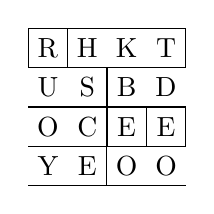
\begin{tikzpicture}[every node/.style={minimum size=.5cm-\pgflinewidth, outer sep=0pt}]
            \draw[step=0.5cm,color=black] (-1,-1) grid (1,1);
            \node[fill=white] at (-0.75,+0.75) {R};
            \node[fill=white] at (-0.25,+0.75) {H};
            \node[fill=white] at (+0.25,+0.75) {K};
            \node[fill=white] at (+0.75,+0.75) {T};
            \node[fill=white] at (-0.75,+0.25) {U};
            \node[fill=white] at (-0.25,+0.25) {S};
            \node[fill=white] at (+0.25,+0.25) {B};
            \node[fill=white] at (+0.75,+0.25) {D};
            \node[fill=white] at (-0.75,-0.25) {O}; 
            \node[fill=white] at (-0.25,-0.25) {C};
            \node[fill=white] at (+0.25,-0.25) {E};
            \node[fill=white] at (+0.75,-0.25) {E};
            \node[fill=white] at (-0.75,-0.75) {Y}; 
            \node[fill=white] at (-0.25,-0.75) {E};
            \node[fill=white] at (+0.25,-0.75) {O};
            \node[fill=white] at (+0.75,-0.75) {O};
        \end{tikzpicture}
    \end{document}
\end{filecontents*}

\begin{filecontents*}{grille2.tex}
    \documentclass{standalone}
    \usepackage{tikz}
    \begin{document}
        
\begin{tikzpicture}[every node/.style={minimum size=.5cm-\pgflinewidth, outer sep=0pt}]
            \draw[step=0.5cm,color=black] (-1,-1) grid (1,1);
            \node[fill=black] at (-0.75,+0.75) {R};
            \node[fill=black] at (-0.25,+0.75) {H};
            \node[fill=black] at (+0.25,+0.75) {K};
            \node[fill=black] at (+0.75,+0.75) {T};
            \node[fill=white] at (-0.75,+0.25) {U};
            \node[fill=black] at (-0.25,+0.25) {S};
            \node[fill=white] at (+0.25,+0.25) {B};
            \node[fill=black] at (+0.75,+0.25) {D};
            \node[fill=black] at (-0.75,-0.25) {O}; 
            \node[fill=black] at (-0.25,-0.25) {C};
            \node[fill=black] at (+0.25,-0.25) {E};
            \node[fill=black] at (+0.75,-0.25) {E};
            \node[fill=white] at (-0.75,-0.75) {Y}; 
            \node[fill=black] at (-0.25,-0.75) {E};
            \node[fill=white] at (+0.25,-0.75) {O};
            \node[fill=black] at (+0.75,-0.75) {O};
        \end{tikzpicture}
    \end{document}
\end{filecontents*}

\begin{filecontents*}{grille3.tex}
    \documentclass{standalone}
    \usepackage{tikz}
    \begin{document}
        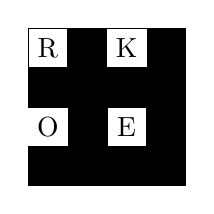
\begin{tikzpicture}[every node/.style={minimum size=.5cm-\pgflinewidth, outer sep=0pt}]
            \draw[step=0.5cm,color=black] (-1,-1) grid (1,1);
            \node[fill=white] at (-0.75,+0.75) {R};
            \node[fill=black] at (-0.25,+0.75) {H};
            \node[fill=white] at (+0.25,+0.75) {K};
            \node[fill=black] at (+0.75,+0.75) {T};
            \node[fill=black] at (-0.75,+0.25) {U};
            \node[fill=black] at (-0.25,+0.25) {S};
            \node[fill=black] at (+0.25,+0.25) {B};
            \node[fill=black] at (+0.75,+0.25) {D};
            \node[fill=white] at (-0.75,-0.25) {O}; 
            \node[fill=black] at (-0.25,-0.25) {C};
            \node[fill=white] at (+0.25,-0.25) {E};
            \node[fill=black] at (+0.75,-0.25) {E};
            \node[fill=black] at (-0.75,-0.75) {Y}; 
            \node[fill=black] at (-0.25,-0.75) {E};
            \node[fill=black] at (+0.25,-0.75) {O};
            \node[fill=black] at (+0.75,-0.75) {O};
            \end{tikzpicture}
    \end{document}
\end{filecontents*}

\begin{filecontents*}{grille4.tex}
    \documentclass{standalone}
    \usepackage{tikz}
    \begin{document}
        
\begin{tikzpicture}[every node/.style={minimum size=.5cm-\pgflinewidth, outer sep=0pt}]
            \draw[step=0.5cm,color=black] (-1,-1) grid (1,1);
            \node[fill=black] at (-0.75,+0.75) {R};
            \node[fill=white] at (-0.25,+0.75) {H};
            \node[fill=black] at (+0.25,+0.75) {K};
            \node[fill=white] at (+0.75,+0.75) {T};
            \node[fill=black] at (-0.75,+0.25) {U};
            \node[fill=black] at (-0.25,+0.25) {S};
            \node[fill=black] at (+0.25,+0.25) {B};
            \node[fill=black] at (+0.75,+0.25) {D};
            \node[fill=black] at (-0.75,-0.25) {O}; 
            \node[fill=white] at (-0.25,-0.25) {C};
            \node[fill=black] at (+0.25,-0.25) {E};
            \node[fill=white] at (+0.75,-0.25) {E};
            \node[fill=black] at (-0.75,-0.75) {Y}; 
            \node[fill=black] at (-0.25,-0.75) {E};
            \node[fill=black] at (+0.25,-0.75) {O};
            \node[fill=black] at (+0.75,-0.75) {O};
        \end{tikzpicture}
    \end{document}
\end{filecontents*}

\begin{filecontents*}{grille5.tex}
    \documentclass{standalone}
    \usepackage{tikz}
    \begin{document}
        
\begin{tikzpicture}[every node/.style={minimum size=.5cm-\pgflinewidth, outer sep=0pt}]
            \draw[step=0.5cm,color=black] (-1,-1) grid (1,1);
            \node[fill=black] at (-0.75,+0.75) {R};
            \node[fill=black] at (-0.25,+0.75) {H};
            \node[fill=black] at (+0.25,+0.75) {K};
            \node[fill=black] at (+0.75,+0.75) {T};
            \node[fill=black] at (-0.75,+0.25) {U};
            \node[fill=white] at (-0.25,+0.25) {S};
            \node[fill=black] at (+0.25,+0.25) {B};
            \node[fill=white] at (+0.75,+0.25) {D};
            \node[fill=black] at (-0.75,-0.25) {O}; 
            \node[fill=black] at (-0.25,-0.25) {C};
            \node[fill=black] at (+0.25,-0.25) {E};
            \node[fill=black] at (+0.75,-0.25) {E};
            \node[fill=black] at (-0.75,-0.75) {Y}; 
            \node[fill=white] at (-0.25,-0.75) {E};
            \node[fill=black] at (+0.25,-0.75) {O};
            \node[fill=white] at (+0.75,-0.75) {O};
        \end{tikzpicture}
    \end{document}
\end{filecontents*}

%%%%% Transposition cipher diagrams %%%%%

\begin{filecontents*}{transpo1.tex}
    \documentclass{standalone}
    \usepackage{tikz}
    \begin{document}
        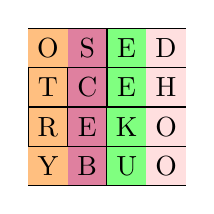
\begin{tikzpicture}[every node/.style={minimum size=.5cm-\pgflinewidth, outer sep=0pt}]
            \draw[step=0.5cm,color=black] (-1,-1) grid (1,1);
            \node[fill=white!50!orange] at (-0.75,+0.75) {O};
            \node[fill=white!50!purple] at (-0.25,+0.75) {S};
            \node[fill=white!50!green] at (+0.25,+0.75) {E};
            \node[fill=white!50!pink] at (+0.75,+0.75) {D};
            \node[fill=white!50!orange] at (-0.75,+0.25) {T};
            \node[fill=white!50!purple] at (-0.25,+0.25) {C};
            \node[fill=white!50!green] at (+0.25,+0.25) {E};
            \node[fill=white!50!pink] at (+0.75,+0.25) {H};
            \node[fill=white!50!orange] at (-0.75,-0.25) {R}; 
            \node[fill=white!50!purple] at (-0.25,-0.25) {E};
            \node[fill=white!50!green] at (+0.25,-0.25) {K};
            \node[fill=white!50!pink] at (+0.75,-0.25) {O};
            \node[fill=white!50!orange] at (-0.75,-0.75) {Y}; 
            \node[fill=white!50!purple] at (-0.25,-0.75) {B};
            \node[fill=white!50!green] at (+0.25,-0.75) {U};
            \node[fill=white!50!pink] at (+0.75,-0.75) {O};
        \end{tikzpicture}
    \end{document}
\end{filecontents*}

\begin{filecontents*}{transpo2.tex}
    \documentclass{standalone}
    \usepackage{tikz}
    \begin{document}
        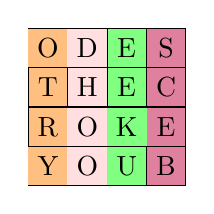
\begin{tikzpicture}[every node/.style={minimum size=.5cm-\pgflinewidth, outer sep=0pt}]
            \draw[step=0.5cm,color=black] (-1,-1) grid (1,1);
            \node[fill=white!50!orange] at (-0.75,+0.75) {O};
            \node[fill=white!50!pink] at (-0.25,+0.75) {D};
            \node[fill=white!50!green] at (+0.25,+0.75) {E};
            \node[fill=white!50!purple] at (+0.75,+0.75) {S};
            \node[fill=white!50!orange] at (-0.75,+0.25) {T};
            \node[fill=white!50!pink] at (-0.25,+0.25) {H};
            \node[fill=white!50!green] at (+0.25,+0.25) {E};
            \node[fill=white!50!purple] at (+0.75,+0.25) {C};
            \node[fill=white!50!orange] at (-0.75,-0.25) {R}; 
            \node[fill=white!50!pink] at (-0.25,-0.25) {O};
            \node[fill=white!50!green] at (+0.25,-0.25) {K};
            \node[fill=white!50!purple] at (+0.75,-0.25) {E};
            \node[fill=white!50!orange] at (-0.75,-0.75) {Y}; 
            \node[fill=white!50!pink] at (-0.25,-0.75) {O};
            \node[fill=white!50!green] at (+0.25,-0.75) {U};
            \node[fill=white!50!purple] at (+0.75,-0.75) {B};
        \end{tikzpicture}
    \end{document}
\end{filecontents*}

\begin{filecontents*}{transpo3.tex}
    \documentclass{standalone}
    \usepackage{tikz}
    \begin{document}
        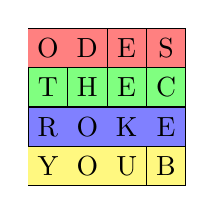
\begin{tikzpicture}[every node/.style={minimum size=.5cm-\pgflinewidth, outer sep=0pt}]
            \draw[step=0.5cm,color=black] (-1,-1) grid (1,1);
            \node[fill=white!50!red] at (-0.75,+0.75) {O};
            \node[fill=white!50!red] at (-0.25,+0.75) {D};
            \node[fill=white!50!red] at (+0.25,+0.75) {E};
            \node[fill=white!50!red] at (+0.75,+0.75) {S};
            \node[fill=white!50!green] at (-0.75,+0.25) {T};
            \node[fill=white!50!green] at (-0.25,+0.25) {H};
            \node[fill=white!50!green] at (+0.25,+0.25) {E};
            \node[fill=white!50!green] at (+0.75,+0.25) {C};
            \node[fill=white!50!blue] at (-0.75,-0.25) {R}; 
            \node[fill=white!50!blue] at (-0.25,-0.25) {O};
            \node[fill=white!50!blue] at (+0.25,-0.25) {K};
            \node[fill=white!50!blue] at (+0.75,-0.25) {E};
            \node[fill=white!50!yellow] at (-0.75,-0.75) {Y}; 
            \node[fill=white!50!yellow] at (-0.25,-0.75) {O};
            \node[fill=white!50!yellow] at (+0.25,-0.75) {U};
            \node[fill=white!50!yellow] at (+0.75,-0.75) {B};
        \end{tikzpicture}
    \end{document}
\end{filecontents*}

\begin{filecontents*}{transpo4.tex}
    \documentclass{standalone}
    \usepackage{tikz}
    \begin{document}
        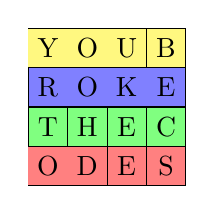
\begin{tikzpicture}[every node/.style={minimum size=.5cm-\pgflinewidth, outer sep=0pt}]
            \draw[step=0.5cm,color=black] (-1,-1) grid (1,1);
            \node[fill=white!50!yellow] at (-0.75,+0.75) {Y};
            \node[fill=white!50!yellow] at (-0.25,+0.75) {O};
            \node[fill=white!50!yellow] at (+0.25,+0.75) {U};
            \node[fill=white!50!yellow] at (+0.75,+0.75) {B};
            \node[fill=white!50!blue] at (-0.75,+0.25) {R};
            \node[fill=white!50!blue] at (-0.25,+0.25) {O};
            \node[fill=white!50!blue] at (+0.25,+0.25) {K};
            \node[fill=white!50!blue] at (+0.75,+0.25) {E};
            \node[fill=white!50!green] at (-0.75,-0.25) {T}; 
            \node[fill=white!50!green] at (-0.25,-0.25) {H};
            \node[fill=white!50!green] at (+0.25,-0.25) {E};
            \node[fill=white!50!green] at (+0.75,-0.25) {C};
            \node[fill=white!50!red] at (-0.75,-0.75) {O}; 
            \node[fill=white!50!red] at (-0.25,-0.75) {D};
            \node[fill=white!50!red] at (+0.25,-0.75) {E};
            \node[fill=white!50!red] at (+0.75,-0.75) {S};
        \end{tikzpicture}
    \end{document}
\end{filecontents*}

%%%%% Main Document %%%%%

\begin{document}

\maketitle

\begin{enumerate}
    \item \textbf{Discuss the difference between Authentication and Authorization.}

        Authentication is ensuring that a user is who they say they are, whereas 
        authorization is enforcing restrictions on a user who is already
        authenticated.

    \item \textbf{What is the plain text of a substitution cipher?}

        \begin{enumerate}[a.]
            \item \textbf{Using a Caesar Cipher with a key of 3 (shift by 3), 
                what is the plaintext if the ciphertext is FUBSWRJUDSKB FDQ EH
                IXQ\@? Work by hand and show all work. Hint: If your solution is
                nonsense, it is probably incorrect.} \\
    
                Since we know the shift number, there are only two possible
                directions to shift: left or right. Knowing that, I've listed
                the two possible plaintexts in the table below. \\

                \begin{align*}
                    \begin{tabular}{@{}lllllllllllllllllllllllllll@{}}
                    \toprule
                    plaintext 1 & x & y & z & a & b & c & d & e & f & g & h & i & j & k & l & m & n & o & p & q & r & s & t & u & v & w \\ \midrule
                        ciphertext  & a & b & c & d & e & f & g & h & i & j & k & l & m & n & o & p & q & r & s & t & u & v & w & x & y & z \\ \midrule
                        plaintext 2 & d & e & f & g & h & i & j & k & l & m & n & o & p & q & r & s & t & u & v & w & x & y & z & a & b & c \bottomrule
                    \end{tabular}
                \end{align*}

                Since the words of the ciphertext are space-delineated, we can
                choose one of the smaller words to attempt to decrypt in order
                to make our lives easier. For this case, I'm going to choose the
                word ``FDQ'' from the ciphertext. \\

                Using plaintext 1: FDQ $\rightarrow$ CAN \\
                Using plaintext 2: FDQ $\rightarrow$ IGT \\

                Since plaintext 1 leaves us with a valid English word, it leads
                me to believe that it is likely the correct answer. \\

                Decrypted: \\
                FUBSWRJUDSKB FDQ EH IXQ
                $\rightarrow$ CRYPTOGRAPHY CAN BE FUN \\

            \item \textbf{Using any means available (Google is your friend) on a
                Substitution Cipher with an unknown key of a random alphabet:}

                \begin{enumerate}
                    \item \textbf{Find the plaintext if the cipher text is:}
                        EXUYGJMJAUVZV ZV RCGWM BZCCZENAG \\

                        Ciphertext: EXUYGJMJAUVZV ZV RCGWM BZCCZENAG \\ 
                        Plaintext: CRYPTANALYSIS IS OFTEN DIFFICULT \\ 

                    \item \textbf{Explain with enough detail to duplicate your
                        method how you solved this.} \\ 

                        Using the website https://quipqiup.com, one can type in
                        ciphertext and the website will generate a list of
                        possible plaintext solutions. In this instance, the fact
                        that the ciphertext was space-delineated greatly
                        improved the solutions that were generated. \\ 

                    \pagebreak

                    \item \textbf{Find the key and explain how you did it (Hint:
                        it will be a mapping of each character used in the
                        cipher text to a corresponding character in the plain
                        text. i.e. A = M, B = Q, etc.).} \\

                        \begin{align*}
                            \begin{tabular}{@{}llllllllllllllll@{}}
                            \toprule
                            ciphertext & a & b & c & e & g & j & m & n & r & u & v & w & x & y & z \\ \midrule
                            plaintext  & l & d & f & c & t & a & n & u & o & y & s & e & r & p & i \\ \bottomrule
                            \end{tabular}
                        \end{align*} \\ \\

                        This mapping was created using the decrypted plaintext.
                        I simply made a set of the unique characters from the
                        ciphertext and found which characters in the plaintext
                        mapped to the characters in the ciphertext.

                \end{enumerate}

        \end{enumerate}

    \item \textbf{Transposition ciphers}

        \begin{enumerate} 
            \item Solve the following Grille cipher using the included cut out.
                Briefly describe your method of breaking the cipher.

                \begin{figure}[H] 
                    \centering
                    \begin{subfigure}[t]{.15\textwidth}
                        \includestandalone{grille1}
                        \caption{Original grid}
                    \end{subfigure}
                    \begin{subfigure}[t]{.15\textwidth}
                        \includestandalone{grille2}
                        \caption{YOUB}
                    \end{subfigure}
                    \begin{subfigure}[t]{.15\textwidth}
                        \includestandalone{grille3}
                        \caption{ROKE}
                    \end{subfigure}
                    \begin{subfigure}[t]{.15\textwidth}
                        \includestandalone{grille4}
                        \caption{THEC}
                    \end{subfigure}
                    \begin{subfigure}[t]{.15\textwidth}
                        \includestandalone{grille5}
                        \caption{ODES}
                    \end{subfigure}
                \end{figure}

                Overlay the grille over the grid, and rotate it four times. With
                each rotation, the order of the ``decrypted'' letters remains
                the same. The caption for each of the above figures is the
                plaintext. Altogether, this reads as \textbf{YOUBROKETHECODES}.

            \item Solve the following Double Transposition cipher. Briefly
                describe your method of breaking the cipher.

                \begin{figure}[H]
                    \centering
                    \begin{subfigure}[t]{.15\textwidth}
                        \includestandalone{transpo1}
                        \caption{Original Order}
                    \end{subfigure}
                    \begin{subfigure}[t]{.15\textwidth}
                        \includestandalone{transpo2}
                        \caption{Col. 2 $\Leftrightarrow$ Col. 4}
                    \end{subfigure}
                    \begin{subfigure}[t]{.15\textwidth}
                        \includestandalone{transpo3}
                        \caption{Reversed rows} 
                    \end{subfigure} 
                    \begin{subfigure}[t]{.15\textwidth}
                        \includestandalone{transpo4}
                        \caption{Final position}
                    \end{subfigure}
                \end{figure}

                I solved this by swapping columns 2 and 4, and then reversing
                all of the resulting rows. This results in the plaintext
                \textbf{YOUBROKETHECODES}. The final key is (4,3,2,1) and
                (1,4,3,2).

        \end{enumerate}

    \item \textbf{What is the one-time pad for encryption?}

        \textbf{Using the letter encoding below discussed in class (along with
            one-time pad using XOR), the ciphertext KITLKE was generated using
            a one-time pad.}

        \textbf{E = 000   H = 001   I = 010   K = 011   L = 100   R = 101   
            S = 110   T = 111}

        \begin{enumerate}[a.]
            \item \textbf{What is the one time pad used if the plain text is ``thrill''?}

                \begin{align*}
                    \begin{tabular}{@{}lllllll@{}}
                        Plaintext          & T   & H   & R   & I   & L   & L   \\
                        Encoded Plaintext  & 111 & 001 & 101 & 010 & 100 & 100 \\ \midrule
                        Ciphertext         & K   & I   & T   & L   & K   & E   \\
                        Encoded Ciphertext & 011 & 010 & 111 & 100 & 011 & 000 \\
                    \end{tabular}
                \end{align*} \\ \\

                Because we have two of the operands of the original XOR
                equation, we can XOR those two operands to find the original
                one-time pad key: \\

                \begin{array}{*{7}c}
                           & \texttt{111} & \texttt{001} & \texttt{101} & \texttt{010} & \texttt{100} & \texttt{100} \\
                    \oplus & \texttt{011} & \texttt{010} & \texttt{111} & \texttt{100} & \texttt{011} & \texttt{000} \\ \hline
                           & \texttt{100} & \texttt{011} & \texttt{010} & \texttt{110} & \texttt{111} & \texttt{100}
                \end{array} \\

                Original one-time pad key: \textbf{100 011 010 110 111 100}, or \textbf{LKISTL}

            \pagebreak

            \item \textbf{What’s the key if the plain text was ``tiller''?}

                \begin{align*}
                    \begin{tabular}{@{}lllllll@{}}
                        Plaintext          & T   & I   & L   & L   & E   & R   \\
                        Encoded Plaintext  & 111 & 010 & 100 & 100 & 000 & 101 \\ \midrule
                        Ciphertext         & K   & I   & T   & L   & K   & E   \\
                        Encoded Ciphertext & 011 & 010 & 111 & 100 & 011 & 000 \\
                    \end{tabular}
                \end{align*} \\ \\

                \begin{array}{*{7}c}
                           & \texttt{111} & \texttt{010} & \texttt{100} & \texttt{100} & \texttt{000} & \texttt{101} \\
                    \oplus & \texttt{011} & \texttt{010} & \texttt{111} & \texttt{100} & \texttt{011} & \texttt{000} \\ \hline
                           & \texttt{100} & \texttt{000} & \texttt{011} & \texttt{000} & \texttt{011} & \texttt{101}
                \end{array} \\

                Original one-time pad key: \textbf{100 000 011 000 011 101}, or \textbf{LEKEKR}

        \end{enumerate}

    \item \textbf{Solve the following null cipher (you do not need to show work or describe how you solved this, but understanding how the answer is derived is still important).}

        BOB RUNS EVERY AFTERNOON\@. KAREN IS NOT GOING\@. CARL ONCE DROVE EVERY
        SUNDAY\@. IRENE SAW HELEN AND ROBERT DANCE\@.

        \textbf{Plaintext:} BREAKINGCODESISHARD

    \item \textbf{BONUS}

        \textbf{Using any means available, find the plaintext for the following
        ciphertext and explain briefly but with enough detail to duplicate your
        method how you solved this:}

        MXDXBVTZWVMXNSPBQXLIMSCCSGXSCJXBOVQXCJZMOJZCVCTVWJCZAAXZBCSSCJXBQCJZCOJZ
        CNSPOXBXSBTVWJCJZDXGXXMOZQMSCSCJXBOVQXCJZMOJZCNSPJZHGXXMOSPLHJZDXZAAXZBX
        HCSCJXTCSGXSCJXBOVQX
        
        \textbf{Plaintext:} ``NEVER IMAGINE YOURSELF NOT TO BE OTHERWISE THAN
        WHAT IT MIGHT APPEAR TO OTHERS THAT WHAT YOU WERE OR MIGHT HAVE BEEN WAS
        NOT OTHERWISE THAN WHAT YOU HAD BEEN WOULD HAVE APPEARED TO THEM TO BE
        OTHERWISE''

        Again, using https://quipqiup.com, this is decrypted rather quickly.
        On this website, it is as simple as pasting in raw ciphertext, clicking
        ``Solve'' and letting the website do it's job. It's remarkably quick and
        accurate.

\end{enumerate}

\end{document}
